\documentclass{beamer}
\usepackage[utf8]{inputenc}
%\usepackage{framed}
%\usepackage{mdframed}
%\usepackage{mathtools}

















\newcommand{\defined}[1]{\textit{#1}}


\RequirePackage{mathtools}
\newcommand{\defeq}{\vcentcolon=}
\newcommand{\eqdef}{=\vcentcolon}

\newcommand{\complexity}[1]{\mathcal{O}(#1)}

\DeclareMathAlphabet{\mymathbb}{U}{bbold}{m}{n}
\newcommand{\neutraladd}[0]{\mymathbb{0}}

\newcommand{\groupaddsym}[0]{\oplus}
\newcommand{\groupadd}[2]{{#1} \groupaddsym {#2}}
\newcommand{\groupsubtract}[2]{{#1} \ominus {#2}}
\newcommand{\inverseadd}[1]{-{#1}}

\newcommand{\abs}[1]{|{#1}|}

\newcommand{\fun}[3]{{#1}: {#2} \rightarrow {#3}}
\newcommand{\set}[1]{\{#1\}}
\newcommand{\disjointunion}[2]{{#1} \dot{\cup} {#2}}
\newcommand{\powerset}[1]{\mathcal{P}({#1})}

\DeclareMathOperator{\lbl}{label}



\usepackage{environ}
\makeatletter
\newsavebox{\measure@tikzpicture}
\NewEnviron{scaletikzpicturetowidth}[1]{%
  \def\tikz@width{#1}%
  \def\tikzscale{1}\begin{lrbox}{\measure@tikzpicture}%
  \BODY
  \end{lrbox}%
  \pgfmathparse{#1/\wd\measure@tikzpicture}%
  \edef\tikzscale{\pgfmathresult}%
  \BODY
}
\makeatother



% domain specific
\DeclareMathOperator{\enc}{enc}
\DeclareMathOperator{\h}{h}
\DeclareMathOperator{\f}{f}
\DeclareMathOperator{\V}{V}

\newcommand{\lift}[2]{\operatorname{lift_{#1}^{#2}}}
\newcommand{\liftlabel}[2]{\operatorname{label_{#1}^{#2}}}

\newcommand{\interval}[3]{[{#1},{#2})_{#3}}
\newcommand{\intervalx}[3]{({#1},{#2})_{#3}}
\newcommand{\fp}[1]{\operatorname{fp}(#1)}
\newcommand{\ifpmanual}[3]{({#1}, {#2}, {#3})}
\newcommand{\ifp}[3]{\ifpmanual{#1}{#2}{\fp{\interval{#1}{#2}{#3}}}}
\newcommand{\iis}[4]{({#1}, {#2}, {#3})_{#4}}
\newcommand{\iisnatural}[4]{({#1}, {#2}, \interval{#1}{#2}{#3}{#4})}
\newcommand{\ifpempty}[2]{({#1}, {#2})}
\newcommand{\ifpsingle}[2]{\ifpmanual{#1}{#2}{\emptyset}}
\newcommand{\ifpcontain}[3]{\ifpmanual{#1}{#2}{\groupadd{\fp{x}}{#3}}}

\newcommand{\successor}[1]{\operatorname{successor({#1})}}

\newcommand{\fpsize}[0]{s_{fp}}
\newcommand{\itemsize}[0]{s_{item}}




\usepackage{tikz}
\usetikzlibrary{arrows.meta}
\usetikzlibrary{shapes}




\newcommand{\examplefp}[1]{#1}
\newcommand{\fpa}[0]{\examplefp{144}}
\newcommand{\fpb}[0]{\examplefp{194}}
\newcommand{\fpc}[0]{\examplefp{240}}
\newcommand{\fpd}[0]{\examplefp{245}}
\newcommand{\fpe}[0]{\examplefp{76}}
\newcommand{\fpf}[0]{\examplefp{221}}
\newcommand{\fpg}[0]{\examplefp{224}}
\newcommand{\fph}[0]{\examplefp{65}}
\newcommand{\fpcd}[0]{\examplefp{229}}
\newcommand{\fpacd}[0]{\examplefp{117}}
\newcommand{\fpefgh}[0]{\examplefp{74}}
\newcommand{\fpbcdh}[0]{\examplefp{232}}
\newcommand{\fpzero}[0]{\examplefp{0}}

%\newcommand{\examplea}[0]{a}
%\newcommand{\exampleb}[0]{b}
%\newcommand{\examplec}[0]{c}
%\newcommand{\exampled}[0]{d}
%\newcommand{\examplee}[0]{e}
%\newcommand{\examplef}[0]{f}
%\newcommand{\exampleg}[0]{g}
%\newcommand{\exampleh}[0]{h}
\newcommand{\examplea}[0]{\ensuremath{\mathrm{ape}}}
\newcommand{\exampleb}[0]{\ensuremath{\mathrm{bee}}}
\newcommand{\examplec}[0]{\ensuremath{\mathrm{cat}}}
\newcommand{\exampled}[0]{\ensuremath{\mathrm{doe}}}
\newcommand{\examplee}[0]{\ensuremath{\mathrm{eel}}}
\newcommand{\examplef}[0]{\ensuremath{\mathrm{fox}}}
\newcommand{\exampleg}[0]{\ensuremath{\mathrm{gnu}}}
\newcommand{\exampleh}[0]{\ensuremath{\mathrm{hog}}}
\newcommand{\examplei}[0]{\ensuremath{\top}}

\newcommand{\hexamplea}[0]{\ensuremath{\h(\mathrm{ape}})}
\newcommand{\hexampleb}[0]{\ensuremath{\h(\mathrm{bee}})}
\newcommand{\hexamplec}[0]{\ensuremath{\h(\mathrm{cat}})}
\newcommand{\hexampled}[0]{\ensuremath{\h(\mathrm{doe}})}
\newcommand{\hexamplee}[0]{\ensuremath{\h(\mathrm{eel}})}
\newcommand{\hexamplef}[0]{\ensuremath{\h(\mathrm{fox}})}
\newcommand{\hexampleg}[0]{\ensuremath{\h(\mathrm{gnu}})}
\newcommand{\hexampleh}[0]{\ensuremath{\h(\mathrm{hog}})}

\newcommand{\aux}[2]{
\begin{tabular}{ c }
{#1} \\ 
\hline
${#2}$
\end{tabular}
}

\tikzset{
aux/.style={
  align=left,
  draw=black,
  fill=white
  }
}

\newcommand{\examplefpi}[3]{
  $\ifpmanual{#1}{#2}{\fp{#3}}$
}
\newcommand{\exampleiis}[4]{
\begin{tabular}{ c | c  | c }
{#1} & {#3} & {#2} \\ 
\end{tabular} $_{(#4)}$
}

\tikzset{
fpi/.style={
  align=left,
  draw=black,
  fill=white
  }
}

\tikzset{
iis/.style={
  align=left,
  draw=black,
  fill=white
  }
}

\tikzset{
local/.style={
  }
}

\tikzstyle{edge} = [draw,thick,opacity=0.25]

\tikzset{%
    %boundingBox/.style={use as bounding box,draw},
    boundingBox/.style={use as bounding box},
    }









%\newcommand{\disjointunion}[2]{{#1} \dot{\cup} {#2}}

\definecolor{cPurple}{RGB}{124, 0, 133}
\definecolor{cBlue}{RGB}{56, 0, 138}
\definecolor{cRed}{RGB}{180, 0, 60}
\definecolor{cGreen}{RGB}{0, 156, 27}

%\newcommand*{\defined}[1]{\textbf{\textcolor{cPurple}{#1}}}

%%%%%%%%%%
% Beamer %
%%%%%%%%%%

\usetheme[sectionpage = none, subsectionpage = simple]{metropolis}
\usecolortheme{seahorse}

\usebeamercolor{normal text}
\usebeamercolor{background canvas}

\setbeamercolor{alerted text}{fg=cPurple}

\setbeamertemplate{footline}{%
      \raisebox{8pt}{\makebox[\paperwidth]{\scriptsize \hspace{5pt}  Recursive Set Reconcilliation \hfill \insertframenumber \hspace{5pt}}}}

\beamertemplatenavigationsymbolsempty

\title[]{Efficient Synchronization of Recursively Partitionable Data Structures}
\date{}

\begin{document}

\frame{\titlepage}

\begin{frame}{Synchronizing Data Structures}
\begin{itemize}
  \item What?
  \begin{itemize}
    \item set reconciliation (aka set union)
    \item set mirroring
    \item map mirroring
  \end{itemize}
  \item Why?
    \begin{itemize}
    \item distributed version control
    \item persistent unordered PubSub
    \item backup creation
    \item update distribution
    \item ...
  \end{itemize}
\end{itemize}
\end{frame}

\begin{frame}{Evaluation Criteria}
\begin{itemize}
\item number of round-trips
\item total bandwidth usage
\item computation time complexity per round-trip
\item space complexity per round-trip
\item space complexity for auxiliary data structures
\item time complexity for keeping auxiliary data structure up to date as the main data structure is being modified
\item soft criteria: simplicity and flexibility
\end{itemize}
\end{frame}

\begin{frame}{Basic Ideas}
\textbf{Divide and conquer}: Let $X_0, X_1$ be sets with $X_0 = \disjointunion{A_0}{B_0}$ and $X_1 = \disjointunion{A_1}{B_1}$, then $X_0 \cup X_1 = (A_0 \cup B_0) \cup (A_1 \cup B_1)$.

\pause
\vspace{24pt}

\textbf{Fingerprints}: Map sets into $\{0, 1\}^{\ast}$ with low probability of collisions. 
\end{frame}

\begin{frame}{Example Protocol Run}
$\examplea < \exampleb < \examplec < \exampled < \examplee < \examplef < \exampleg < \exampleh < \examplei$

$X_0 \defeq \{\exampleb, \examplec, \exampled, \examplee, \examplef, \exampleh \}$
\hfill
$X_1 \defeq \{\examplea, \examplee, \examplef, \exampleg\}$


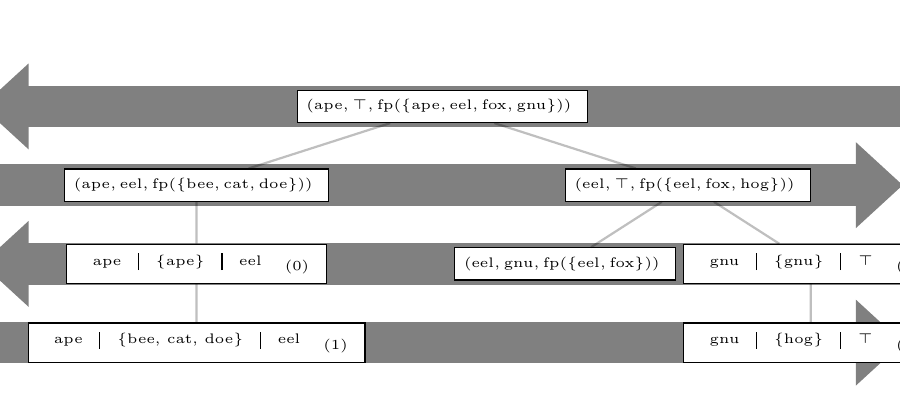
\begin{tikzpicture}[xscale=0.78, yscale=1.0, font=\tiny]
        \path[boundingBox] (-6.75,-2.5) rectangle (7,2);
        
	\pgfdeclarelayer{background}
	\pgfdeclarelayer{foreground}
	\pgfsetlayers{background,main,foreground}
	
	\begin{pgfonlayer}{main}
		%vertices
		\node (vroot) at (0, 1) [fpi] {\examplefpi{\examplea}{\examplei}{\{\examplea, \examplee, \examplef, \exampleg\}}};
		
		\pause

		\node (v00) at (-4, -0) [fpi] {\examplefpi{\examplea}{\examplee}{\{\exampleb, \examplec, \exampled\}}};
		\draw (vroot) edge[edge] (v00);
		\node (v01) at (4, -0) [fpi] {\examplefpi{\examplee}{\examplei}{\{\examplee, \examplef, \exampleh\}}};
                \draw (vroot) edge[edge] (v01);
		\pause

                \node (v10) at (-4, -1) [iis] {\exampleiis{\examplea}{\examplee}{\{\examplea\}}{0}};
                \draw (v00) edge[edge] (v10);
                \pause
                \node (v11) at (2, -1) [fpi] {\examplefpi{\examplee}{\exampleg}{\{\examplee, \examplef\}}};
                \node (v12) at (6, -1) [iis] {\exampleiis{\exampleg}{\examplei}{\{\exampleg\}}{0}};
                \draw (v01) edge[edge] (v11);
		\draw (v01) edge[edge] (v12);
		\pause

                \node (v20) at (-4, -2) [iis] {\exampleiis{\examplea}{\examplee}{\{\exampleb, \examplec, \exampled\}}{1}};
                \node (v21) at (6, -2) [iis] {\exampleiis{\exampleg}{\examplei}{\{\exampleh\}}{1}};
                \draw (v10) edge[edge] (v20);
		\draw (v12) edge[edge] (v21);
	\end{pgfonlayer}
	
	\begin{pgfonlayer}{background}		\draw[-{Triangle[width=30pt,length=17pt,color=gray]}, line width=15pt, color=gray](7.5, 1) -- (-7.5, 1);
		\draw[-{Triangle[width=30pt,length=17pt,color=gray]}, line width=15pt, color=gray](-7.5, -0) -- (7.5, -0);
		\draw[-{Triangle[width=30pt,length=17pt,color=gray]}, line width=15pt, color=gray](7.5, -1) -- (-7.5, -1);
		\draw[-{Triangle[width=30pt,length=17pt,color=gray]}, line width=15pt, color=gray](-7.5, -2) -- (7.5, -2);
	\end{pgfonlayer}
\end{tikzpicture}
\end{frame}

\begin{frame}{A Worst-Case Run}
$X_0 \defeq \{\examplea, \examplec, \examplee, \exampleg \}$
\hfill
$X_1 \defeq \{\examplea, \exampleb, \examplec, \exampled, \examplee, \examplef, \exampleg, \exampleh\}$

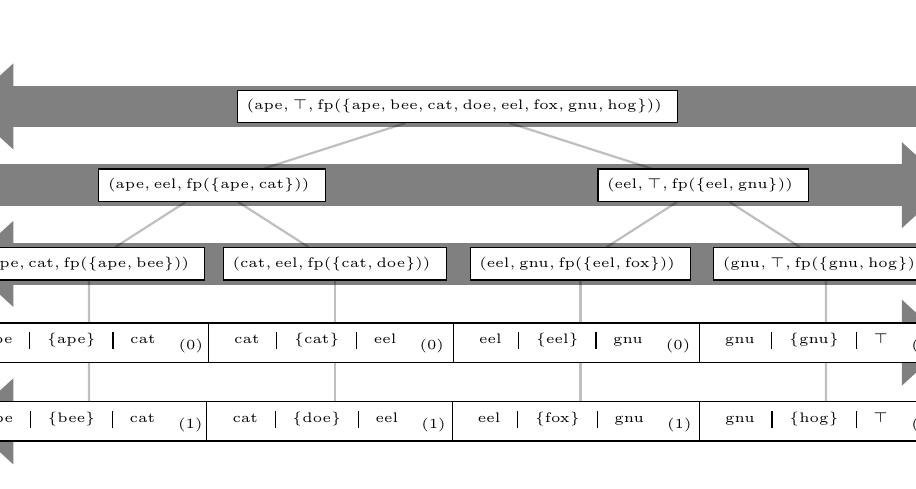
\begin{tikzpicture}[xscale=0.78, yscale=1.0, font=\tiny]
        \path[boundingBox] (-7,-3.5) rectangle (7,2);
	\pgfdeclarelayer{background}
	\pgfdeclarelayer{foreground}
	\pgfsetlayers{background,main,foreground}
	
	\begin{pgfonlayer}{main}
		%vertices
		\node (vroot) at (0, 1) [fpi] {\examplefpi{\examplea}{\examplei}{\{\examplea, \exampleb, \examplec, \exampled, \examplee, \examplef, \exampleg, \exampleh\}}};

		\node (v00) at (-4, -0) [fpi] {\examplefpi{\examplea}{\examplee}{\{\examplea, \examplec\}}};
		\node (v01) at (4, -0) [fpi] {\examplefpi{\examplee}{\examplei}{\{\examplee, \exampleg\}}};

                \node (v10) at (-6, -1) [fpi] {\examplefpi{\examplea}{\examplec}{\{\examplea, \exampleb\}}};
                \node (v11) at (-2, -1) [fpi] {\examplefpi{\examplec}{\examplee}{\{\examplec, \exampled\}}};
                \node (v12) at (2, -1) [fpi] {\examplefpi{\examplee}{\exampleg}{\{\examplee, \examplef\}}};
                \node (v13) at (6, -1) [fpi] {\examplefpi{\exampleg}{\examplei}{\{\exampleg, \exampleh\}}};

                \node (v20) at (-6, -2) [iis] {\exampleiis{\examplea}{\examplec}{\{\examplea\}}{0}};
                \node (v21) at (-2, -2) [iis] {\exampleiis{\examplec}{\examplee}{\{\examplec\}}{0}};
                \node (v22) at (2, -2) [iis] {\exampleiis{\examplee}{\exampleg}{\{\examplee\}}{0}};
                \node (v23) at (6, -2) [iis] {\exampleiis{\exampleg}{\examplei}{\{\exampleg\}}{0}};

                \node (v30) at (-6, -3) [iis] {\exampleiis{\examplea}{\examplec}{\{\exampleb\}}{1}};
                \node (v31) at (-2, -3) [iis] {\exampleiis{\examplec}{\examplee}{\{\exampled\}}{1}};
                \node (v32) at (2, -3) [iis] {\exampleiis{\examplee}{\exampleg}{\{\examplef\}}{1}};
                \node (v33) at (6, -3) [iis] {\exampleiis{\exampleg}{\examplei}{\{\exampleh\}}{1}};
		%edges
                \draw (vroot) edge[edge] (v00);
                \draw (vroot) edge[edge] (v01);

		\draw (v00) edge[edge] (v10);
		\draw (v00) edge[edge] (v11);
		\draw (v01) edge[edge] (v12);
		\draw (v01) edge[edge] (v13);

		\draw (v10) edge[edge] (v20);
		\draw (v11) edge[edge] (v21);
		\draw (v12) edge[edge] (v22);
		\draw (v13) edge[edge] (v23);

		\draw (v20) edge[edge] (v30);
		\draw (v21) edge[edge] (v31);
		\draw (v22) edge[edge] (v32);
		\draw (v23) edge[edge] (v33);
	\end{pgfonlayer}
	
	\begin{pgfonlayer}{background}
		\draw[-{Triangle[width=30pt,length=17pt,color=gray]}, line width=15pt, color=gray](8, 1) -- (-8, 1);
		\draw[-{Triangle[width=30pt,length=17pt,color=gray]}, line width=15pt, color=gray](-8, -0) -- (8, -0);
		\draw[-{Triangle[width=30pt,length=17pt,color=gray]}, line width=15pt, color=gray](8, -1) -- (-8, -1);
		\draw[-{Triangle[width=30pt,length=17pt,color=gray]}, line width=15pt, color=gray](-8, -2) -- (8, -2);
		\draw[-{Triangle[width=30pt,length=17pt,color=gray]}, line width=15pt, color=gray](8, -3) -- (-8, -3);
	\end{pgfonlayer}
\end{tikzpicture}
\end{frame}

\begin{frame}{A \textit{Different} Worst-Case Run}
$X_0 \defeq \{\examplea, \exampleb, \examplec, \exampled, \examplee, \exampleg, \exampleh \}$
\hfill
$X_1 \defeq \{\examplea, \exampleb, \examplec, \exampled, \examplee, \examplef, \exampleg, \exampleh \}$

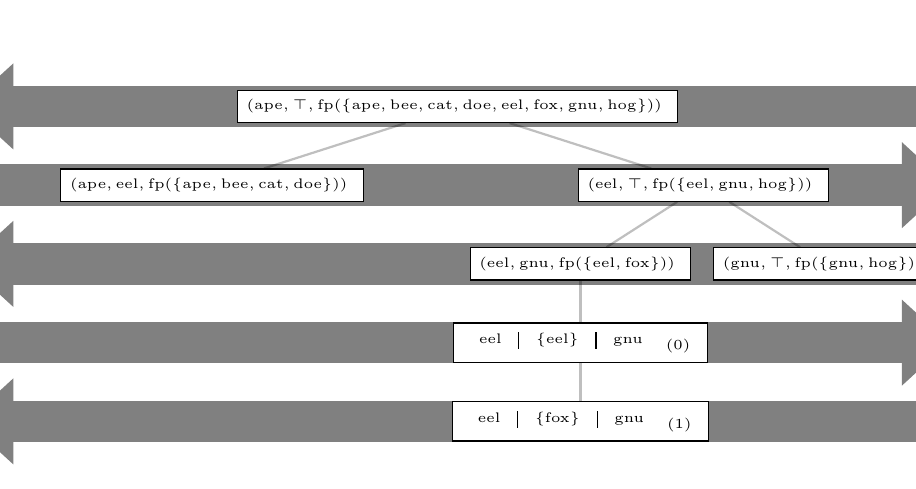
\begin{tikzpicture}[xscale=0.78, yscale=1.0, font=\tiny]
        \path[boundingBox] (-7,-3.5) rectangle (7,2);
	\pgfdeclarelayer{background}
	\pgfdeclarelayer{foreground}
	\pgfsetlayers{background,main,foreground}
	
	\begin{pgfonlayer}{main}
		%vertices
		\node (vroot) at (0, 1) [fpi] {\examplefpi{\examplea}{\examplei}{\{\examplea, \exampleb, \examplec, \exampled, \examplee, \examplef, \exampleg, \exampleh\}}};

		\node (v00) at (-4, -0) [fpi] {\examplefpi{\examplea}{\examplee}{\{\examplea, \exampleb, \examplec, \exampled\}}};
		\node (v01) at (4, -0) [fpi] {\examplefpi{\examplee}{\examplei}{\{\examplee, \exampleg, \exampleh\}}};

                \node (v10) at (2, -1) [fpi] {\examplefpi{\examplee}{\exampleg}{\{\examplee, \examplef\}}};
                \node (v11) at (6, -1) [fpi] {\examplefpi{\exampleg}{\examplei}{\{\exampleg, \exampleh\}}};

                \node (v20) at (2, -2) [iis] {\exampleiis{\examplee}{\exampleg}{\{\examplee\}}{0}};

                \node (v30) at (2, -3) [iis] {\exampleiis{\examplee}{\exampleg}{\{\examplef\}}{1}};

		%edges
                \draw (vroot) edge[edge] (v00);
                \draw (vroot) edge[edge] (v01);

		\draw (v01) edge[edge] (v10);
		\draw (v01) edge[edge] (v11);

		\draw (v10) edge[edge] (v20);
		
		\draw (v20) edge[edge] (v30);
	\end{pgfonlayer}
	
	\begin{pgfonlayer}{background}
		\draw[-{Triangle[width=30pt,length=17pt,color=gray]}, line width=15pt, color=gray](8, 1) -- (-8, 1);
		\draw[-{Triangle[width=30pt,length=17pt,color=gray]}, line width=15pt, color=gray](-8, -0) -- (8, -0);
		\draw[-{Triangle[width=30pt,length=17pt,color=gray]}, line width=15pt, color=gray](8, -1) -- (-8, -1);
		\draw[-{Triangle[width=30pt,length=17pt,color=gray]}, line width=15pt, color=gray](-8, -2) -- (8, -2);
		\draw[-{Triangle[width=30pt,length=17pt,color=gray]}, line width=15pt, color=gray](8, -3) -- (-8, -3);
	\end{pgfonlayer}
\end{tikzpicture}
\end{frame}

\end{document}
